\documentclass[a4paper,11pt,utf8]{scrartcl}

\usepackage[ngerman]{babel}
\usepackage[utf8]{inputenc}
\usepackage[a4paper, left=2cm, right=2cm, top=1.5cm, bottom=1.5cm]{geometry}
\usepackage{graphicx}
\usepackage{stmaryrd}
\usepackage{listings}
\usepackage{amsmath}
\usepackage[hidelinks]{hyperref}
\usepackage[onehalfspacing]{setspace}

\setlength{\headsep}{.5cm}

\begin{document}

\pagestyle{empty}

% Titlepage
\noindent
Praktikum: Big Data \hfill Klemens Schölhorn, Sebastian Lange, Simon Hüning \hfill 04.02.2016\vspace{-.4cm}\\
\begin{center}
\huge\textsf{Lösungsskizze zum zweiten Testat}\vspace{.1cm}\\
\large Zitierungsanalyse auf den Daten der DBLP unter Verwendung von Apache Kylin
\end{center}

\section*{Einleitung}

Die ersten drei Abschnitte beschreiben die bisher umgesetzten Arbeiten, während in Sektion \ref{sec:plan} der Plan für die noch ausstehenden Tätigkeiten dargelegt wird.

\section{Server}

\subsection{Software}

Auf dem für das Praktikum zur Verfügung gestellten Rechner \texttt{wdi06} wurde basierend auf dem im installierten Ubuntu 14.04 LTS enthaltenen opendjk-7 folgende Software installiert:

\begin{itemize}
    \item Hadoop (HDFS): 2.7.1
    \item HBase: 0.98.15
    \item Hive: 0.14.0
    \item Kylin: 1.1
    \item Flink 0.10.1
\end{itemize}

\noindent
Es konnten aufgrund von Beschränkungen von Kylin\footnote{\url{http://kylin.incubator.apache.org/docs/install/index.html}} keine aktuellen Versionen von HBase und Hive verwendet werden. Es existiert zwar eine Version von Kylin für HBase 1.1.3, letzteres wurde jedoch noch nicht offiziell veröffentlicht.

\subsection{Einrichtung}

Die Hadoop-Umgebung wurde im pseudo-verteilten Modus installiert, d.\,h. es werden die gleichen Knoten wie in einer verteilten Umgebung verwendet, jedoch alle auf einer physischen Maschine und nur jeweils eine Instanz pro Knotentyp.

Die Installation erfolgte ohne root-Rechte in einem Benutzerverzeichnis durch Setzen der benötigten Umgebungsvariablen (\texttt{HADOOP\_HOME}, \texttt{HBASE\_HOME}, $\dots$). Dabei wurde weitgehend auf die Standard-Konfiguration gesetzt und nur die minimal benötigte Konfiguration vorgenommen.\footnote{Details dazu finden sich im Installationsprotokoll im privaten Repository: \texttt{Installation.txt}}

Da die meisten Dienste standardmäßig an allen Adressen (und damit auch der öffentlichen Adresse) lauschen, wurde zusätzlich die in Ubuntu integrierte Firewall \texttt{ufw} aktiviert.

\section{Datenbankschema}

Das folgende vorläufige Datenbankschema basiert auf dem in der Aufgabenstellung vorgeschlagenen und wurde nur an einigen Stellen geringfügig angepasst. Einige der Schlüssel werden voraussichtlich keine Ganzzahlen, sondern Zeichenketten sein.

\noindent
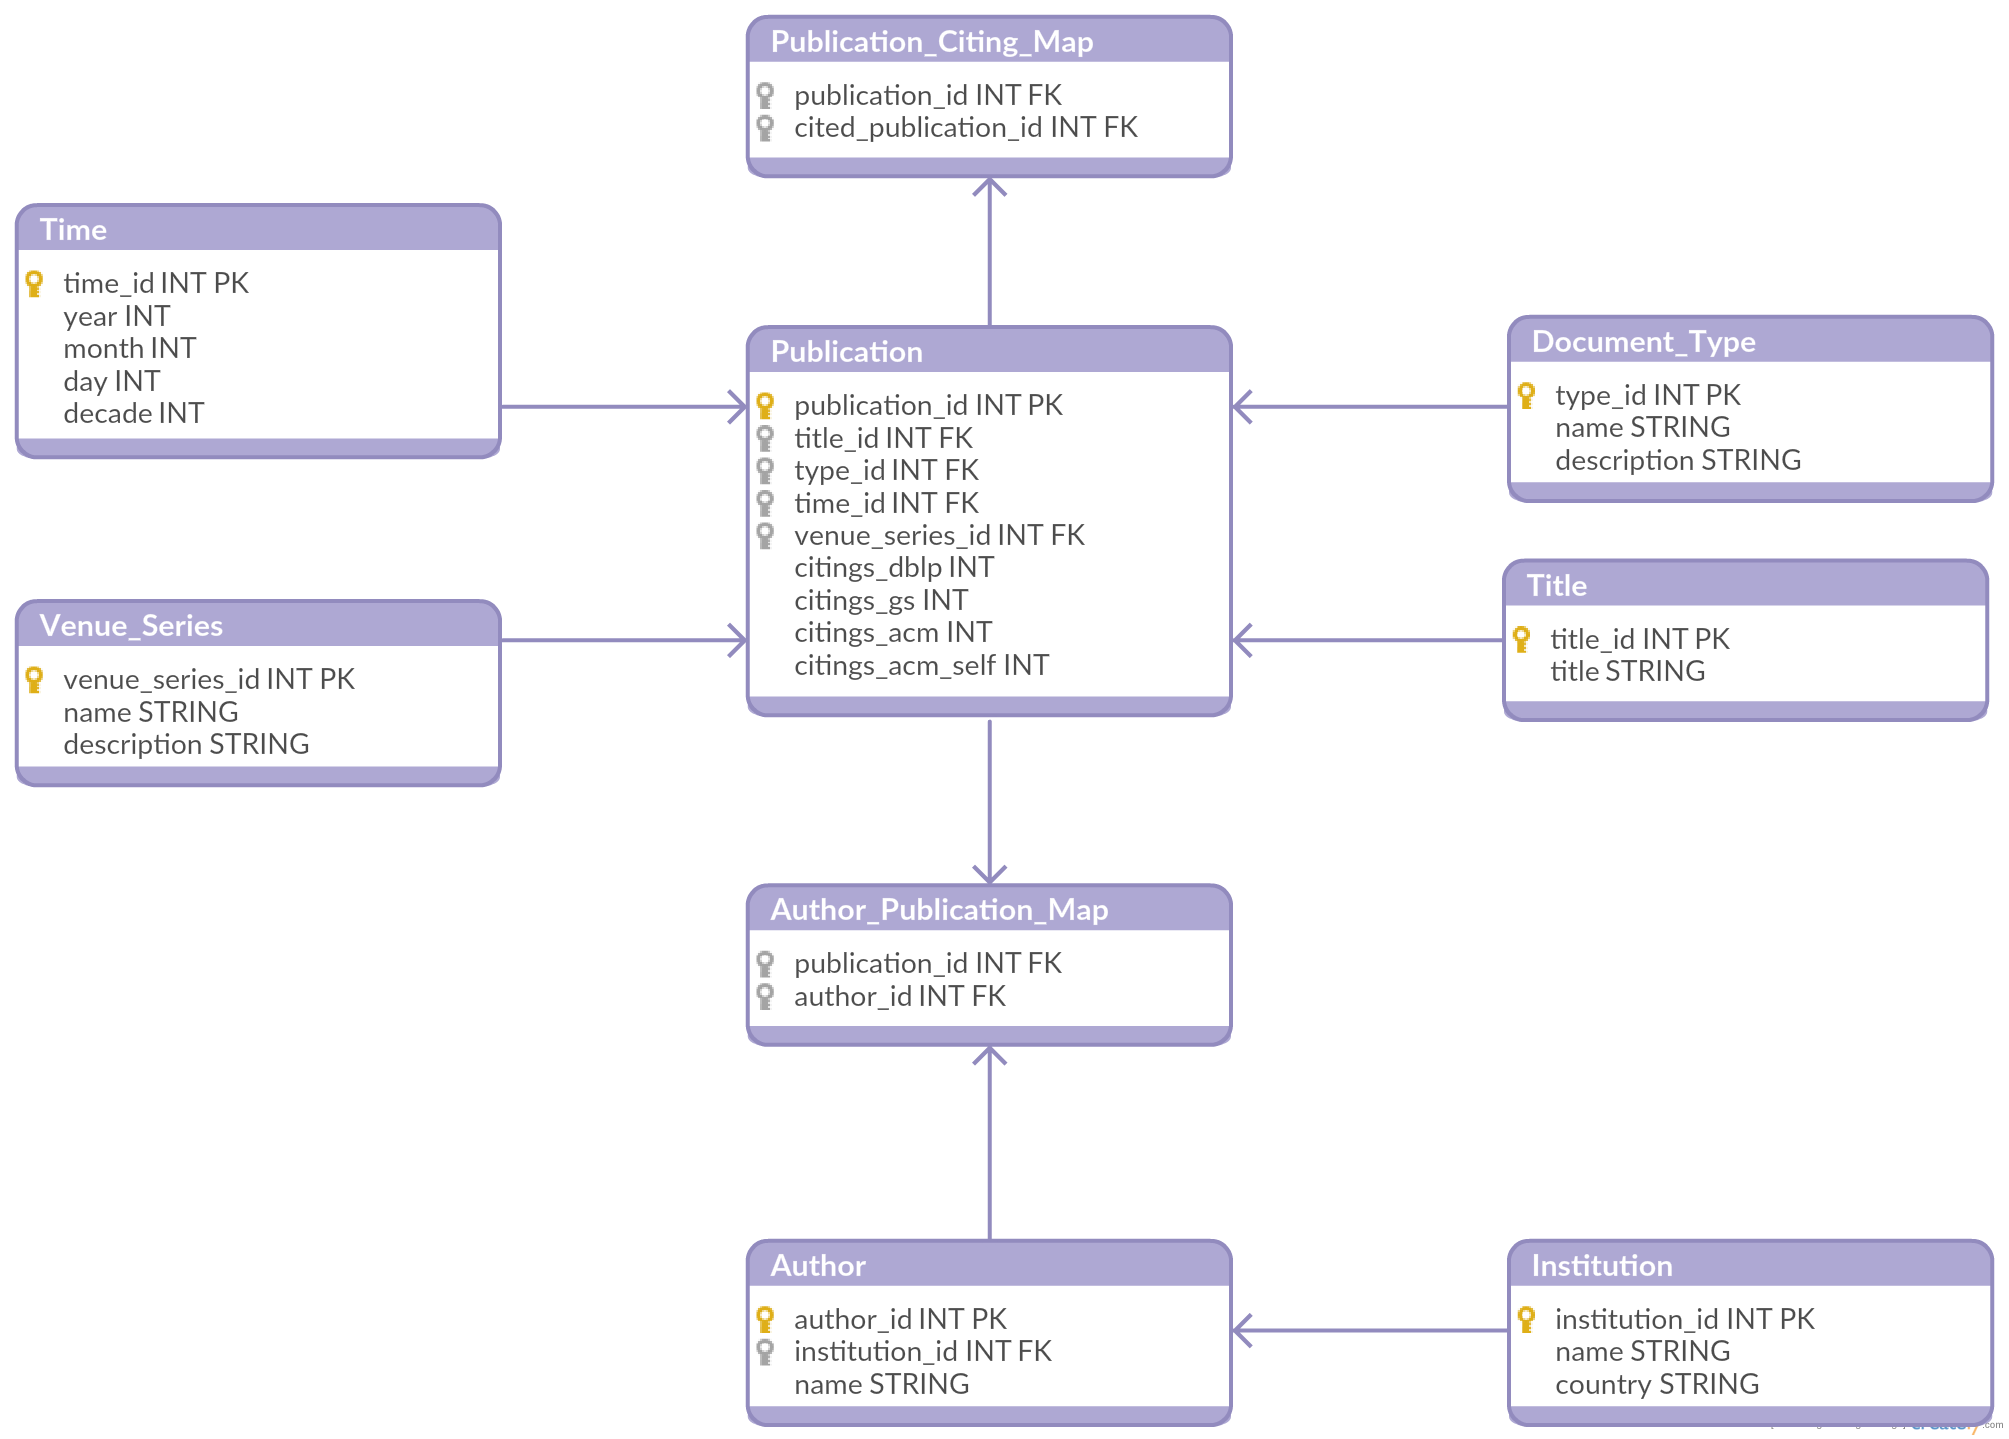
\includegraphics[width=\textwidth]{pics/schema.png}

\begin{itemize}
    \item \texttt{Publication\_Citing\_Map}: Zitat einer Publikation (nicht Teil des endgültigen Sternschemas)
    \item \texttt{Publication}: Zitierungszahlen werden aus \texttt{Publication\_Citing\_Map} generiert
    \item \texttt{Document\_Type}: Typ der Publication, z.\,B. Journal, Artikel, Kollektion
\end{itemize}

\section{Datenimport}

Der Import der Daten gestaltete sich aufgrund der Datengröße schwierig. So kann die \texttt{dblp.xml} nicht direkt mit einem DOM-Parser verarbeitet werden, da dafür zu viel Speicher benötigt wird. Aus diesem Grund muss ein SAX- oder StaX-Parser verwendet werden.

Auch ein direkter Import per MapReduce stellte sich als schwierig heraus, da immer komplette XML-Records gelesen werden müssen, was der standardmäßig zeilenweisen Verarbeitung von MapReduce widerspricht. Hadoop besitzt zwar einen \texttt{StreamXmlRecordReader}, der jedoch selbst in aktuellen Versionen scheinbar nicht immer problemlos funktioniert\footnote{\url{https://issues.apache.org/jira/browse/MAPREDUCE-577}}.

Alternativ wird oft \texttt{XmlInputFormat} von Mahout (einem Hadoop-basierten Machine-Learning-Tool) verwendet\footnote{\url{http://oobaloo.co.uk/articles/2010/1/20/processing-xml-in-hadoop.html}}, was diese Probleme nicht hat. Allerdings müssen dabei alle zu lesenden Records das gleiche XML-Tag verwenden, was bei der \texttt{dblp.xml} leider nicht der Fall ist.

Aus diesem Grund haben wir ein eigenes Tool für den Import entwickelt. Der \texttt{pub-importer}\footnote{\url{https://github.com/klemens/bigdata-kylin-dblp}} liest die \texttt{dblp.xml} aus einer Datei oder von \texttt{stdin}, verwendet StAX für das Parsen und schreibt das Ergebnis anschließend direkt ins HDFS. Dabei ist unabhängig von der Größe der Eingabedatei der Speicherverbrauch konstant.

Die exportierten Daten werden dabei in einem zu Hive (oder alternativ zu unserem \texttt{dblp-formatter}) kompatiblen Format geschrieben (CSV mit Backslash als Escape-Zeichen oder mit Anführungszeichen versehen) und bestehen aus zwei Dateien: Einmal die \texttt{Collections} wie Konferenzberichte oder Bücher und schließlich die \texttt{Publications} an sich mit entsprechenden Verweisen auf die \texttt{Collections}.

Zusätzlich kann der \texttt{pub-importer} auch den im Data-Warehouse-Praktikum verwendeten, unvollständigen xml-Dump von ACM lesen und auf die gleiche Weise ins HDFS schreiben. Da dort jedoch keine Informationen über die Journals enthalten sind, entfällt hierbei die \texttt{Collections}-Datei.

\subsection{Probleme bei der Datentransformation mit PDI}

Bei der Umsetzung der Datentransformation mit PDI kam es zu einigen Problemen. Ein Problem ist die Implementierung des OUTER-JOIN in PDI. Diese Implementierung arbeitet nicht wie erwartet. Dies könnte daran liegen, dass die OUTER-JOIN Logik ausschließlich als Merge-JOIN implementiert ist. Da sich dieses Problem mit einigem Aufwand umgehen lässt, ist die Umsetzung der Tranformation mit PDI daran letztlich nicht gescheitert. Dafür jedoch an den folgenden Problemen.

PDI hat bei der Umsetzung stets sämtliche Schritte (Vergleich, Sortierung, Merge, etc.) parallel im Arbeitsspeicher ausgeführt. Es war daher auch mit 12 GB RAM nicht möglich alle Transformation auf der gesamten Datenmenge durchzuführen. Nach Laufzeiten von bis zu vier Stunden war das Ergebnis immer nur eine Exception. Für kleine Datenmengen hingegen funktionierte die selbe Transformation tadellos.

Darüber hinaus stellte sich während der Umsetzung heraus, dass die in PDI designten Transformationen nicht ohne weiteres auf dem Server ausführbar sind. Diese müssen (insofern kein zusätzlicher Deployment-Prozess dafür implementiert wird) auf dem Server immer an mehreren Stellen neu konfiguriert und angepasst werden, bevor sie ausführbar sind. Je komplexer die Transformation ist, umso umfangreicher sind die nötigen Anpassungen. Zusätzlich zu diesen Einschränkungen ist es alles andere als trivial, die Ausführung der Transformationen so zu konfigurieren, dass die Vorteile eines vorhandenen Clusters vollständig ausgenutzt werden.

Aus diesen Gründen ist das Verhältnis zwischen Aufwand und Nutzen sehr schlecht. Daher wurde die Datentransformation nicht, wie ursprünglich geplant, mit PDI umgesetzt.

\subsection{Datentransformation mit Apache Flink}

Nach den Problemen mit PDI wurde die Datentransformation in das Sternschema mittels Apacha Flink implementiert, woraus dann der \texttt{dblp-formatter} entstand.

Allerdings gab es auch hier einige Komplikationen: Das Problem ist die Verwendung von zwei verschiedenen CSV-Implementierungen, einmal der CSVReader von Apache Commons und dann der CSVReader von Apache Flink, wobei sich letzterer an keinerlei Standards (RFC 4180) hält und sich auch nicht ausreichend konfigurieren lässt. So unterstützt er nur die Quoting-Variante zum Speichern von CSVs. Allerdings erwartet er nicht wie üblich eine Verdopplung des Quoting-Zeichens, wenn dieses innerhalb eines Strings auftaucht, sondern erwartet das Escaping des Quoting-Zeichens mit einem Backslash, was weder dem Standard entspricht, noch mit dem CSVWriter von Apache Commons ausgegeben werden kann.

Abgesehen von diesem Problem läuft der Transformationsvorgang reibungslos. So werden zuerst die Dimensionstabellen erzeugt, indem die nötigen Felder aus den importierten Dateien in neue CSV-Dateien projiziert werden. Jeder Eintrag in den Tabellen ist dabei eindeutig. Die Faktentabelle entsteht anschließend durch einen Join der Dimensionstabellen. Der gesamte Vorgang dauert auf den dblp-Daten ca. zehn Minuten.

\section{Plan}
\label{sec:plan}

\subsection{Definieren der externen Hive-Tabellen}

Nach Abschluss des Datenverarbeitungsschrittes, bei dem die Daten mit dem \texttt{dblp-formatter} in einzelne CSV-Dateien überführt werden, werden darauf entsprechende externe Hive-Tabellen definiert, um den Zugriff aus Kylin zu ermöglichen. Dies ist aktuell bereits größtenteils umgesetzt.

\subsection{Cube-Generierung mit Kylin}

Wenn die Tabellen in Hive definiert sind, sollte die Generierung der Cubes in Kylin relativ einfach möglich sein. Dies soll bis Mitte Februar erfolgen.

\subsection{Analyse der Daten aus den Cubes}

Nach der Generierung der Cubes sollen darauf u.\,a. die in der Aufgabenstellung beschrieben Abfragen ausgeführt werden. Dies soll bis spätestens 1 Woche vor der Vorstellung der Ergebnisse am 4. März 2016 erfolgen.

\end{document}
